\chapter{Background and State of the Art}
This chapter serves as an overview of the current state of the art regarding low-cost teleoperative surgical training systems. This section will explore their architecture, advantages, and disadvantages. Additionally, this section will delve into current control standards and strategies that these systems use and will discuss the ROS 2 and its applications.

\section{The da Vinci Research Kit}  
The da Vinci Research Kit (dVRK) is a research platform developed through a collaboration between academic institutions, Johns Hopkins University and Worcester Polytechnic Institute, and Intuitive Surgical Inc. in 2012. It consists of first-generation da Vinci components that allow for a common development platform between institutions for the research of robotic-assisted surgery. The dVRK consists of two da Vinci MTMs, two da Vinci PSMs, a stereo viewer, a foot pedal tray, manipulator interface boards (dMIBs), and a basic accessory kit. \cite{DVRKComponents}

At the time of writing in 2025, the dVRK program has been used by 40 research centers in 10 countries \cite{DVRKRTD}. It offers a high-performance platform for researchers using hardware that would otherwise be retired. However, it is not without its disadvantages. The system has a very large footprint; three different pieces of large capital equipment are required by this system, and it is not easily transportable. Additionally, the system is expensive to acquire and maintain, creating a high barrier to entry for many applications. Because of these limitations, researchers recognized the need for additional options in the surgical robotics research space. This ultimately resulted in the Raven II \cite{6363574}.

\begin{figure}[H]
    \centering
    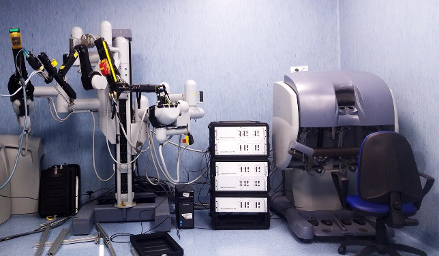
\includegraphics[width=0.75\linewidth]{figures/DVRK.png}
    \caption{The Original Da Vinci Research Kit.(Reprinted from \cite{Fontanelli2017ModellingAI} Fig 1)}
    \label{fig:DVRK}
\end{figure}



\section{The Raven II Surgical System}

The \textbf{Raven II} is an open-architecture robotic surgical system developed by the University of Washington and the University of California, Santa Cruz. It is a low-cost alternative to the dVRK and draws much design inspiration from the original da Vinci's capstan cable drive system. The Raven II is a continuation of the original Raven system and was designed to be as modular as possible to make the system more portable than existing surgical systems. The Raven II system consists of two cable-driven PSMs, a cable-driven Mantis Duo MTM, a stereoscopic surgeon viewer, and control electronics


Each of the Raven II's 7-DOF arms are remotely driven by a cable system powered by brushless DC motors. Encoders are directly coupled to the motors, which leads to difficulties in state estimation. Cable stretch and linkage flexure lead to discrepancies between the actual joint angles and the motor output. This design can be seen in \textbf{Figure \ref{fig:ravenII_design}}.

\begin{figure}[h!]
    \centering
    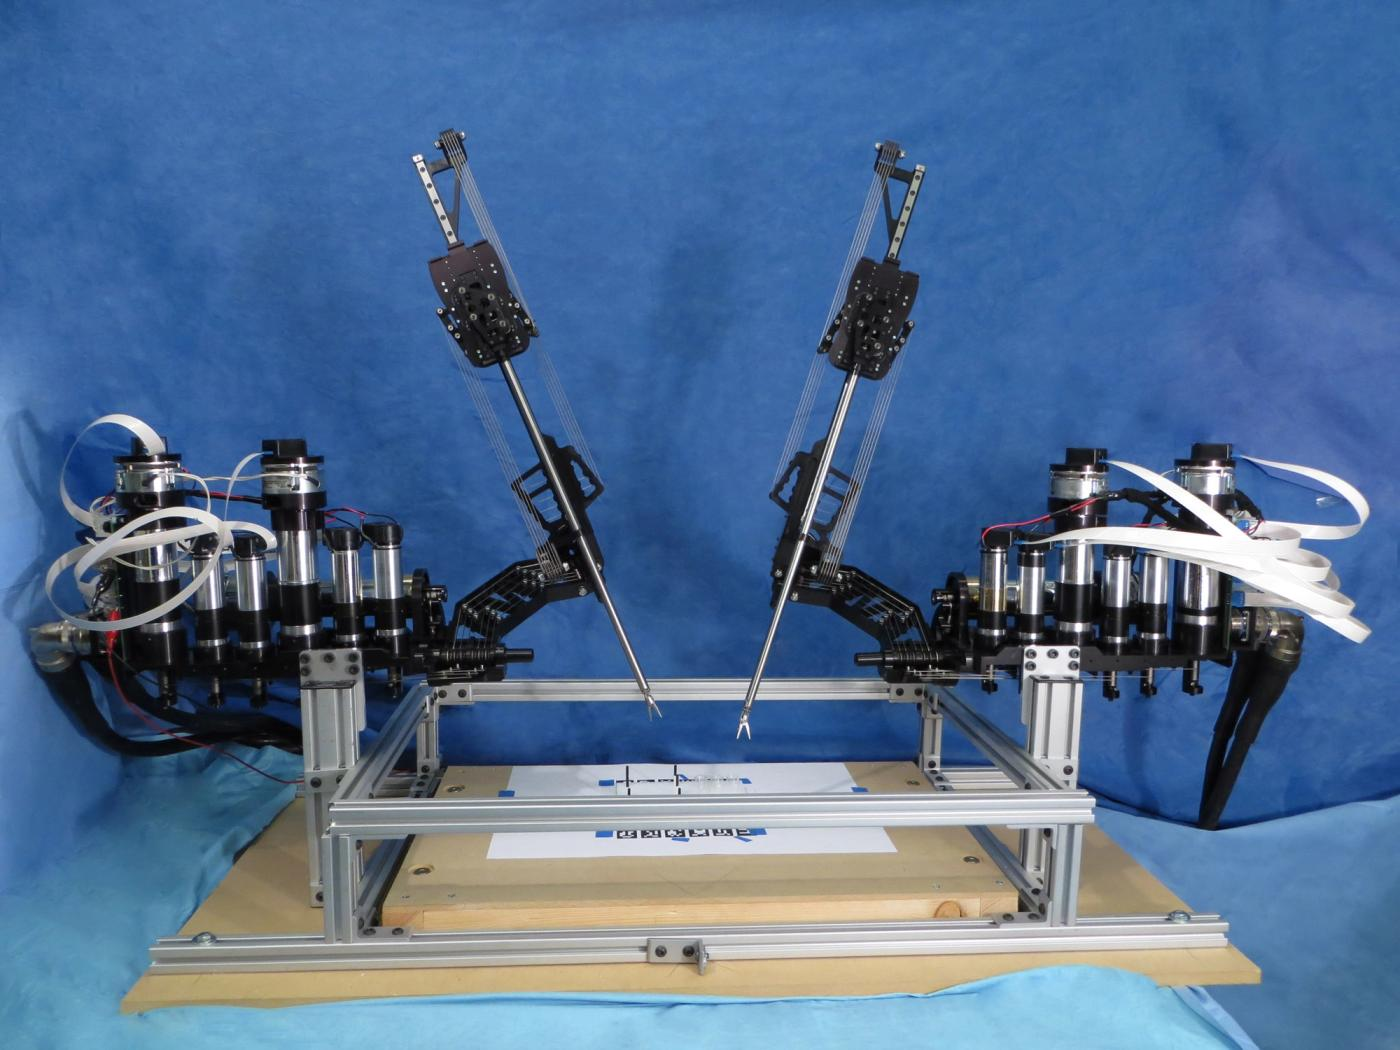
\includegraphics[width=1.0\linewidth]{figures/raven_II.jpg}
    \caption{The Raven II surgical system design. In this figure the cable driven design can clearly be seen (Reprinted from \cite{Hannaford2013RavenII} Fig 1)}
    \label{fig:ravenII_design}
\end{figure}

The Raven II is driven by the Mantis Duo. The MTM design features a novel approach where each MTM is suspended by four driven cables. These cables allow for simultaneous positional sensing of the surgeon's movements while providing haptic feedback.

While the Raven II is a smaller alternative to the dVRK, it still requires a significant investment in hardware, costing \$250,000 USD \cite{RobotsGuideRaven} for a complete system. This cost remains prohibitive for many research institutions and limits the system's accessibility.
\section{Robot Operating System}

Robot Operating System 2 (ROS 2) is a Linux-based, open-source robotics middleware suite consisting of software frameworks for robotic applications. ROS 2 is a direct evolution of ROS 1 and improves upon many aspects. While ROS 1 relied on a centralized ROS Master, ROS 2 uses the Data Distribution Service (DDS) for decentralized, peer-to-peer communication, eliminating the single point of failure present in the master node and increasing system reliability. ROS 2 also provides full real-time performance and supports most common microcontrollers through Micro-ROS, which is critical for many modern applications.

ROS 2 has proven itself as an industry standard, being utilized frequently in cutting-edge applications such as autonomous vehicles, humanoid robotics, and even surgical robotics \cite{Chen2013OpenSource}. Its suite of tools and utilities provides researchers with valuable development resources, including system visualization, collision detection, and frame transformation libraries, all of which are valuable assets to a Robotic Autonomous System.


\begin{figure}[H]
    \centering
    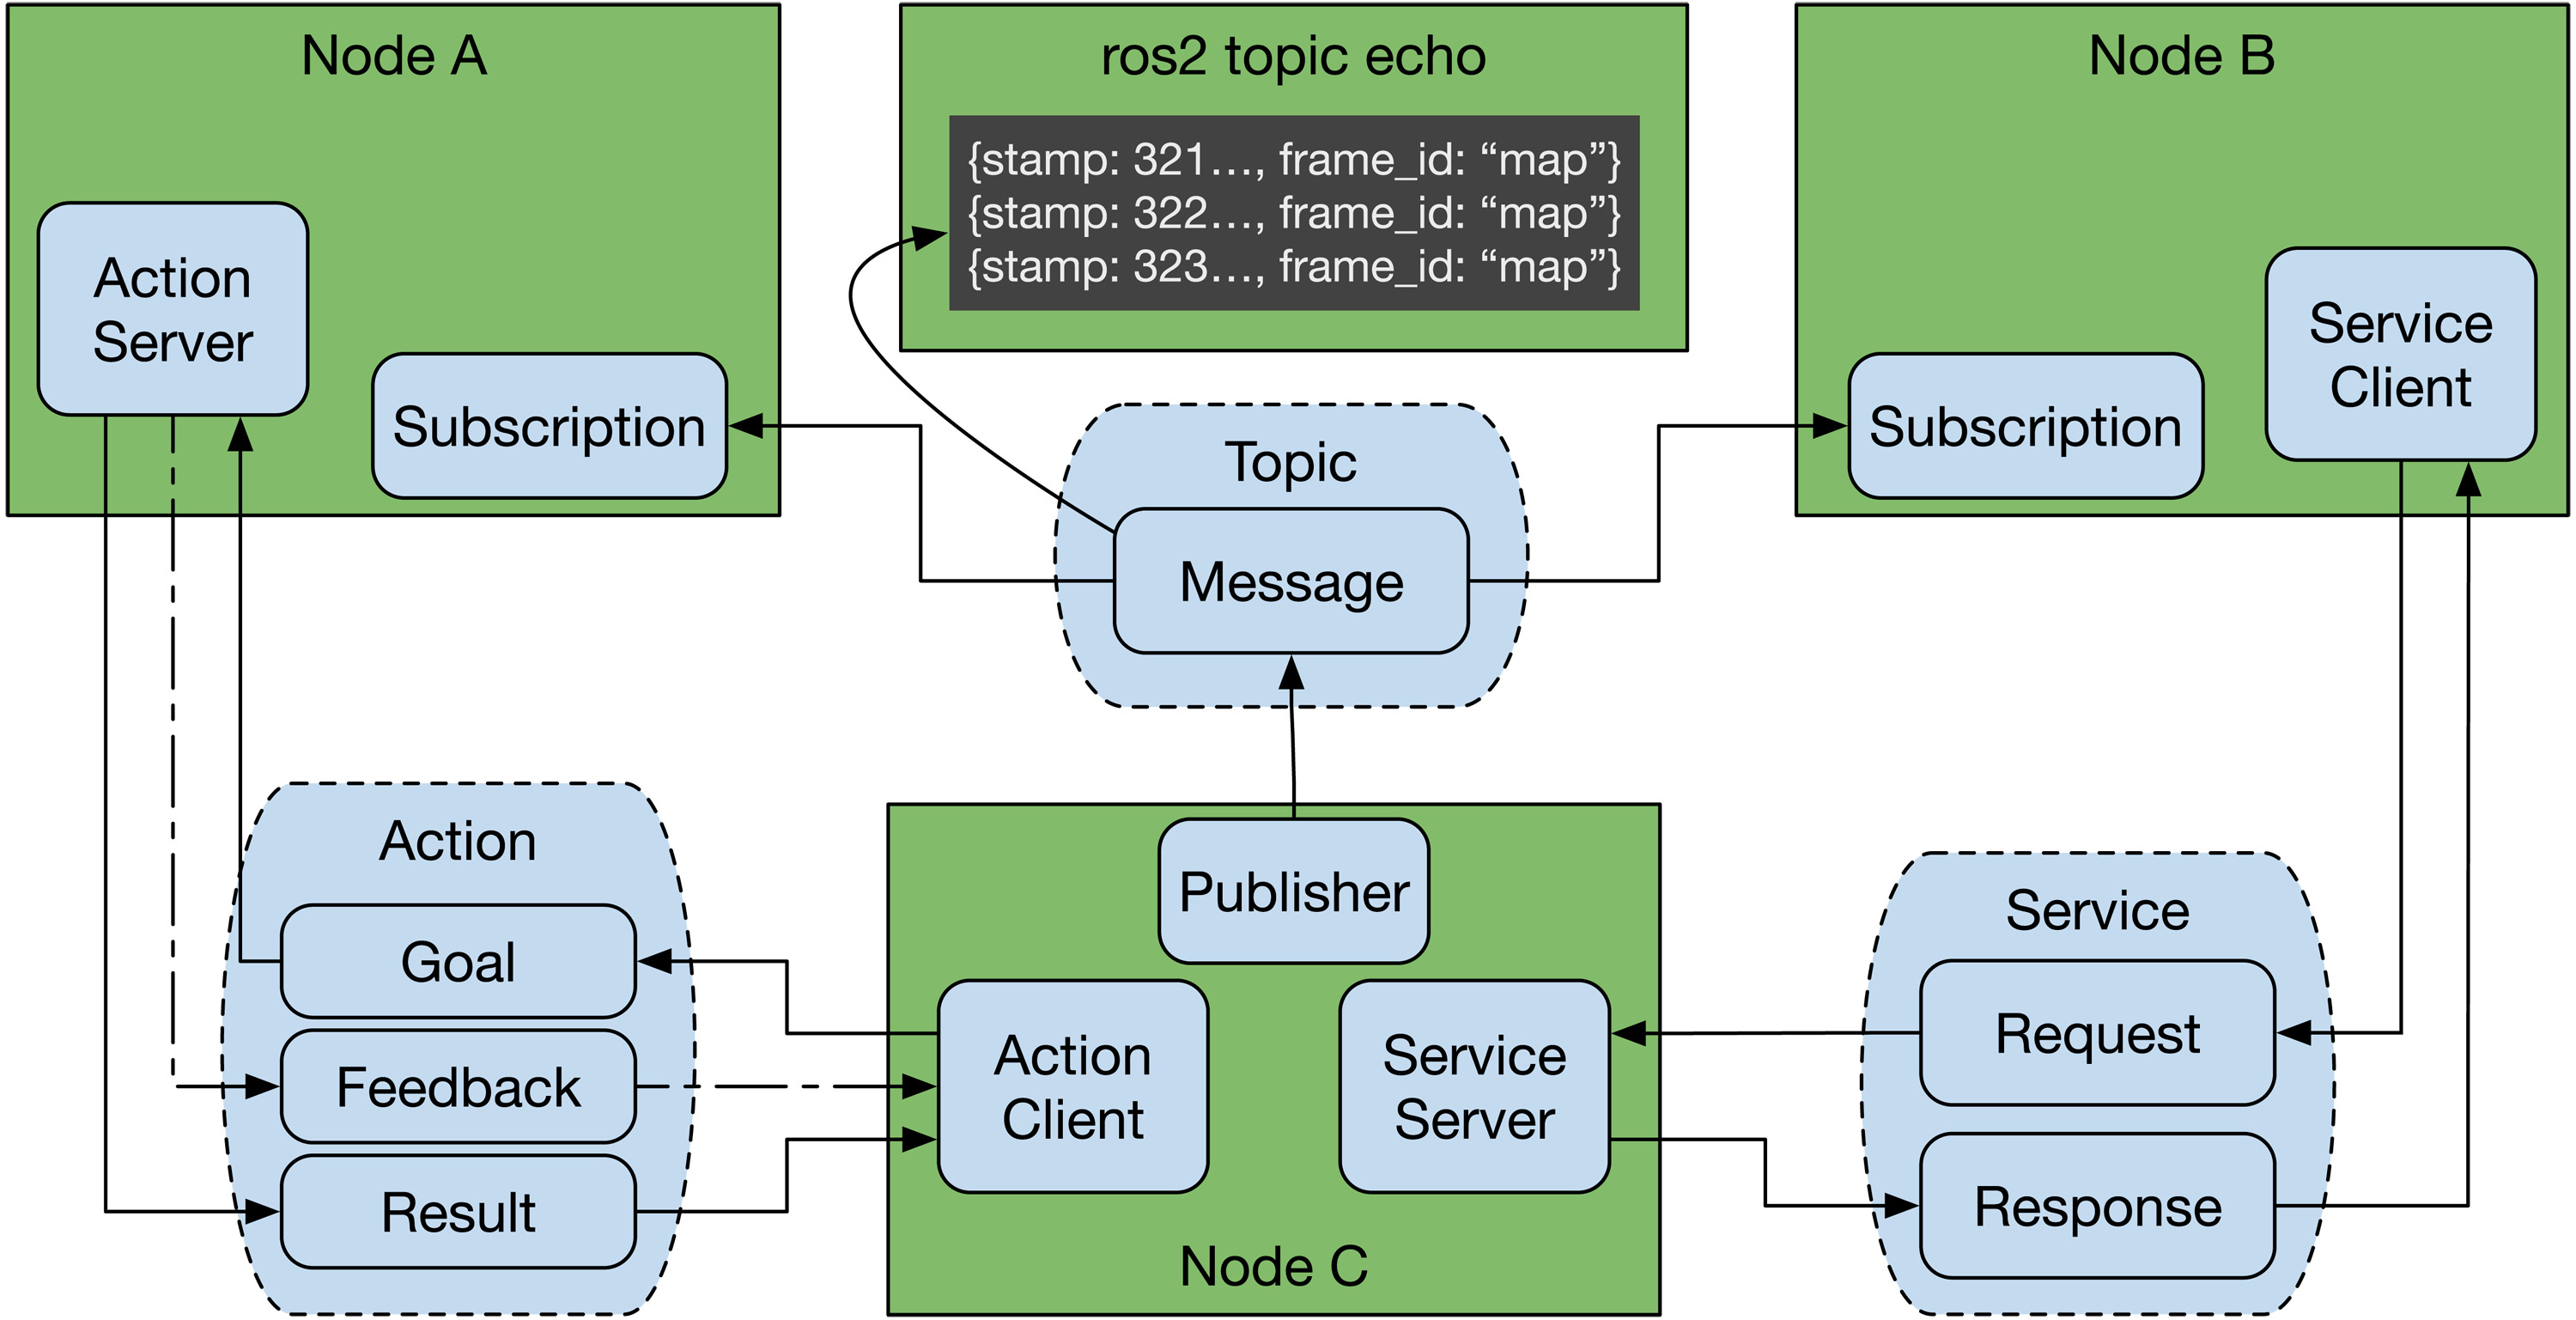
\includegraphics[width=1\linewidth]{figures/ROS2.png}
    \caption{An overview of a typical ROS 2 node network consisting of subscription nodes and publishing nodes, actions and service types can also be seen (Reprinted from \cite{doi:10.1126/scirobotics.abm6074} Fig 2)}
    \label{fig:ROS2}
\end{figure}


\section{Control Techniques in Robotic Surgery}

Precise control, haptic feedback, complex system dynamics, and high safety standards drive the need for sophisticated control techniques in modern robotic surgery systems. Industry-leading platforms such as Intuitive Surgical's da Vinci system utilize Model Predictive Control (MPC) \cite{Kazanzides2014DVRK}, enabling comprehensive modeling and prediction of system behavior. These systems also employ hierarchical control architectures (combining high-level planning with low-level execution) along with adaptive learning-based controllers to compensate for tissue deformation and operate effectively in dynamic environments.

Surgeon feedback is equally critical for successful surgical outcomes. Advanced haptic feedback and force control algorithms are implemented in master-tool manipulators (MTMs) to provide surgeons with precise tactile information \cite{Okamura2001HapticSurgery}. Furthermore, real-time imaging and navigation systems deliver valuable intraoperative feedback to enhance surgical precision \cite{Maier2015ImageGuidedSurgery}. The integration of artificial intelligence has revolutionized surgical robotics in recent years. Deep learning approaches now enable advanced perception and decision-making capabilities within these systems. For instance, real-time tissue identification \cite{Wang2020DeepLearningTissue} allows for dynamic force modeling, enabling systems to adapt intelligently to varying tissue properties during procedures.

\section{System Identification Techniques in Robotic Surgery}

Implementing advanced control strategies requires a dynamic understanding of system behavior, which can only be achieved through robust system identification. The highly nonlinear nature of many robotic systems demands excitation methods that remain effective under nonlinear conditions. Multisine and chirp signals form the basis for many modern system identification techniques \cite{Xia1997ChirpSignals}, and are increasingly combined with reinforcement learning approaches \cite{MARTINSEN20208130}. In surgical robotics, where safety is paramount, a multi-stage identification process is critical. For example, Intuitive Surgical performs low-level actuator characterization using step-response tests to validate settling time, overshoot, and stiffness in every motor and joint. These physics-based models are then enhanced with AI/ML layers to handle complex surgical interactions. This hybrid approach delivers uncompromising system dynamics and performance \cite{US20230309921A1}.

\section{Summary and Research Motivation}

Modern robotic-assisted surgical systems provide a powerful framework to assist doctors and surgeons, enabling them to improve patient quality of care while reducing postoperative recovery time. While these systems are incredibly capable, their high cost and barriers to entry have limited accessibility for researchers. This limitation has led to the development of several lower-cost alternatives, such as the Da Vinci Research Kit, Raven II, and the Desktop Surgical System.

These systems inherit many features found in commercial solutions, including a ROS-based architecture and advanced control and identification techniques. However, the gap between their implementation and the current state of the art remains apparent. This research aims to reduce this technical gap by, upgrading the software architecture to ROS 2, implementing more advanced system identification techniques, and incorporating adaptive control to improve system performance.